\section{Cookbooks}
\label{sec:cookbooks}

In this section, we will present a number of "cookbooks" - example of how to use \foam in typical or less tipical ways.


\subsection{How to set up computations}

\subsection{Simple setups}

\subsubsection{1D horizontal and vertical models}
Here we perform a series of one-dimensional examples with constant temperature and pressure conditions, these conditions are the same as what in \cite{weis2014hydrothermal}.

\begin{figure}[!h]
	\centering
	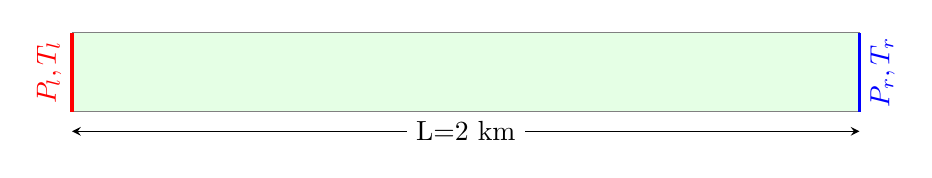
\begin{tikzpicture}[scale=5,>=stealth]
\def\xmin{0}
\def\xmax{2}
\def\ymin{0}
\def\ymax{0.2}

\filldraw[gray,fill=green,fill opacity=0.1] (\xmin,\ymin) -- (\xmax,\ymin) -- (\xmax,\ymax) -- (\xmin,\ymax)  --cycle;

\draw[red,very thick] (\xmin, \ymin) -- (\xmin, \ymax) node[pos=0.5, rotate=90, above] {$P_l, T_l$};

\draw[blue,very thick] (\xmax, \ymin) -- (\xmax, \ymax) node[pos=0.5, rotate=90, below] {$P_r, T_r$};

\draw[black,<->] (\xmin,\ymin-0.05) -- (\xmax, \ymin-0.05) node[pos=0.5,fill=white] {L=2 km};
\end{tikzpicture}
	\caption{1D Model geometry}
\end{figure}

\begin{table}[htbp]
	\centering
	\begin{threeparttable}
		\caption{Boundary conditons of 1-D models}
		\label{tab:conditions_1Dmodels}
		\begin{tabular}{lllll}
			\toprule
			Model Index & Boundary condition left/bottom & Boundary condition right/top & Initial condition & End time \\
			\midrule
			1 &  350\ssd, 50 MPa & 150 \ssd, 25 MPa & 150 \ssd  & 250, 750 year\\
			2 &  450\ssd, 40 MPa & 300 \ssd, 20 MPa & 300 \ssd  & 120, 350 year\\
			3 &  500\ssd, 15 MPa & 350 \ssd, 1 MPa & 350 \ssd  & 1500 year\\
			\bottomrule
		\end{tabular}
	\end{threeparttable}
\end{table}

\begin{table}[htbp]
	\centering
	\begin{threeparttable}
		\onehalfspacing
		\caption{Transport parameters of 1-D models}
		\label{tab:transportParms_1D}
		\begin{tabular}{llllll}
			\toprule
			Parameter & Symbol & Unit & Value & Variable Name& Location \\
			\midrule
			Permeability & $k$ & $m^2$ & $10^{-15}$ & \mintinline{bash}{permeability} & 0/permeability \\
			Porosity & $\phi$ & $1$ & $0.1$ & \mintinline{bash}{porosity} & constant/transportProperties \\
			Heat capacity of rock & $c_{pr}$ & $\frac{J}{kg ^{\circ}\text{C}}$ & $880$ & \mintinline{bash}{cp_rock} & constant/transportProperties \\
			Thermal conductivity of rock & $K_r$ & $\frac{W}{m ^{\circ}\text{C}}$ & $2$ & \mintinline{bash}{kr} & constant/transportProperties \\
			Density of rock & $\rho_r$ & $\frac{kg}{m^3}$ & $2700$ & \mintinline{bash}{rho_rock} & constant/transportProperties \\
			\bottomrule
		\end{tabular}
	\begin{tablenotes}[para,flushleft]
		The temperature value should be transformed from Celsius to Kelvin, e.g. 350 \ssd = 350+273.15=623.15 K .
	\end{tablenotes}
	\end{threeparttable}
\end{table}

\begin{figure}
	\centering
	\includegraphics[width=0.7\textwidth]{cookbooks/1D_Weis2014}
	\caption{Temperature and pressure distribution of 1D models}
\end{figure}

\subsubsection{2D box}

\subsection{2D pipe model without reaction}

\subsection{2D pipe model with reaction}

\subsection{2D model of hydrothermal system with detachment}

\subsection{3D pipe model}


